\documentclass{article}
\usepackage[utf8]{inputenc}

\usepackage{array}
\usepackage{wrapfig}
\usepackage{multirow}
\usepackage{tabularx}
\usepackage{tikz}
\usepackage[T1]{fontenc}
\usepackage{amsmath}
\usepackage{float}
%Margenes
\usepackage{geometry}
\addtolength{\hoffset}{-.5cm}
\addtolength{\textwidth}{.8cm}
\addtolength{\voffset}{-0.5cm}
\addtolength{\textheight}{1.9cm}

\title{Heurística: Proyecto 1 \\ Facultad de Ciencias UNAM 2021-I }
\author{Ruiz Melo Jean Paul}
\date{Noviembre 13th}

\begin{document}

\maketitle
    %%%%%%%%%%%%%%%%%%%%%%%%%%%%%%%%%%%%%%%%%%%%%%%%%%%%%%%%%%%%%%%%%%%%%%%%%%%%%%%%%%%%%%%%%%%%%%%%%%%%%%%%%
    \section{Introducción}
    % Introducción (el problema TSP, la heurística de SA con TA) %
    El problema del agente viajero (or TSP) consiste en resolver la siguiente problema:
    \begin{center}
    ``Dado un subconjunto de ciudades en un mapa, ¿cuál es el camino más corto que pasa por todas ellas (si
    acaso existe)?" 
    \end{center}\\ 
    
    Dado una gráfica G, con V el conjunto de todo las ciudades y E el conjunto de aristas con peso igual
    a la distancia entre ellos, queremos encontrar la distancia optima para recorre a todos una vez. Para este
    proyecto, si dos ciudades u y v no tienen una conexión, entonces le proponemos uno para ellos.
    Esta distancia le llamos la distancia natural y se define como:
    
    \begin{center}
        d(u, v) = 6,373,000 $\times$ 2 $\times$ $arctan(\sqrt{A},\sqrt{1-A})$
    \end{center} 
        Donde A se define como:
    \begin{center}
        A = sin$^{2}$( $\frac{lat(v) - lat(u)}{2}$) + cos(lat(u)) $\times$ cos(lat(v)) $\times$ sin$^{2}$($\frac{lon(v) - lon(u)}{2}$)
    \end{center}
    
    La distancia natural es entonces multiplicado por la arista de peso máximo que existe en G. Esto nos deja
    asegurar que todo solución que contiene una conexión entre dos ciudades que no existe tiene un peso
    mucho mayor a uno que esta en la gráfica. Para entonces encontrar un camino que si es posible existir
    definimos un función de costo. El función de costo toma la distancia entre cada ciudad en el camino i y i+1.
    \\
    
   % This natural distance is then multiplied by the maximum connection that already exists within the graph. This allows
    %us to insure that any path that contains a connection that isn't in the graph is heavily skewed. To find the actual
    %shortest path however we'll use a cost function. This cost function will take the distance between every two cities
    %i and i+1. However, we also wish to be able to know which paths are possible as well. \\
    
    De esto, tambien calculamos un normal para saber que camino si es posible o no. Para hacer esto debemos
    dividir por un normal. Este normal lo podemos definir como la suma de las |S - 1| distancias más grandes
    en la gráfica, donde |S| es igual al número de ciudades en el camino. Con esto normal cuando dividimos el
    funcion de costo podemos saber lo siguiente:\\
\begin{itemize}
    \item Si el resultado del funcion de costo es mayor que 1, el resultado no es factible ya que contine
    una arista con la distancia natural
    \item Si es menor que 0, entonces es factible. Lo mas cercano a 0 mejor es la respuesta
\end{itemize}
    %%To accomplish this we'll normalize the cost function result versus the worst \textit{possible} path available. To do 
    %this we'll simply divide by the sum of the |S - 1| greatest distances in the graph, where |S| is equal to the number
    %of cities. With this normal, we can simply divide the cost function result. If the result is now greater than 1, then
    %the result is simply not feasible as it's worse than the already worst path. If it is less than 1 then we know it is
    %a possible path, as we heavily skewed non-existence paths with the natural distance.\\
    
    Definiendo un funcion de costo podemos empezar a encontrar una solucion usando la Heurística de
    Recocido Simulado. Mientras que encontrando la solucion más optima tardaria mucho, podemos acercarnos
    a ese solucion. Recocido Simulado se base en acercar a la solucion global minima usando un proceso
    de enfriamiento lento que es interpretado como un decaimiento lento en la probabilidad de
    aceptar una solucion peor en el espacio explorado. Aceptando soluciones malas propone un mejor busqueda
    de la solucion minima en el espacio explorado.
    %We can begin attempting to find a solution using the Heuristic Simulated Annealing. While finding the perfect 
    %solution would take too long, we can approximate the next best thing. Simulated annealing allows us to approach a
   % global minimum. This is done through a process of slow cooling which is interpreted as a slow
    %decreases in the probability of accepting worse solutions as the solution space is explored.
    %Accepting worse solutions allows for a more extensive search for the global optimal solution.\\
    
    Para empezar tenemos que definir una temperatura. Una temperatura muy alto resula en tiempo perdido
    ya que la mejora de la solucion actual empieza a ser minuscula. Pero una temperatura muy baja puede resultar
    en atorarse en una minima local. Para encontrar una temperatura mejor hacemos una busqueda binaria donde
    nos basamos en aceptar una gran cantidad de soluciones, pero no todas. \\
     %To begin however, we have to select a temperature. A temperature that's too high will result in wasted time as the
     %improvement in solutions becomes practically minuscule. A temperature that's too low will result in finding a local
     %minimum, and thus get trapped in a worse solution that we could have achieved. To do this we'll do a binary search
    % where we accept a large amount of solutions, but not all of them. \\
    
    La heurística propia es basado en lotes de soluciones. Dado un numero L que nosotros definimos, generamos
    soluciones nuevos hasta que encontramos L numero de soluciones que fueron mejores que el anterior. Seguimos
    generando lotes hasta que el promedio del función de costo de lotes generaros es mayor que el promedio
    del lote anterior. Bajamos la temperatura con enfriamiento y empezamos a generar lotes de nuevo hasta
    que la temperatura llega a un punto determinado por nosotros. Podemos garantizar que este proceso termina
    proponiendo un maximo de soluciones posibles de generar por Lote. \\
    
   %  The heuristic itself is based off of lots of paths or solutions. Given a number L that we wish to meet, we generate
    % any number of neighbor solutions until we have L that are better than the previous neighbor. By returning the average
    % sum of the cost function we can decide when it is prudent to lower the temperature or not. We define a neighbor
    % as a solution that had two of it's cities swapped. We can guarantee this process stops by setting a large number of
    % neighbor generations before we return the average of what we currently have. \\
    
    Finalmente, durante el proceso guardamos un minimo global, este minimo global es el solucion que se va a
    proporner al final.
    % Additionally, by keeping track of a global minimum, we can return the best solution that we found. As long as the
    % cost function result of this solution is less than 1, we know it is feasible. \\
    
    %%%%%%%%%%%%%%%%%%%%%%%%%%%%%%%%%%%%%%%%%%%%%%%%%%%%%%%%%%%%%%%%%%%%%%%%%%%%%%%%%%%%%%%%%%%%%%%%%%%%%%%%%%
    \section{Tecnologías usadas}\\
    % Un recuento de las tecnologías que decidieron usar; C++ con Meson; Rust con Cargo; etc., junto con una justificación de porqué tomaron esa decisión. %
    \begin{itemize}
        \item {Lenguage de programacion: Originalmente este proyecto fue hecho en rust, pero debido a problemas con conectando al base de datos el lenguaje se cambio a Java por la comidad y costumbre a aquel.}
        \item{Compilador: ANT fue usado por el mismo razon dado anteriormente}
        \item{Imagenes: Gnuplot fue usado para generar las graficas}
    \end{itemize}

   %Programming Language: Originally the project was meant to have been done in rust. However issues with
   %connections to the data base resulted in scrambling for a different language. To make up for last time
   %the project was done in Java due to comfort. \\
   
   %Compiler: ANT was used to help compile and connect to the database using SQLite \\
   
   %Images: Gnuplot was used to graph resulting paths. \\
    %%%%%%%%%%%%%%%%%%%%%%%%%%%%%%%%%%%%%%%%%%%%%%%%%%%%%%%%%%%%%%%%%%%%%%%%%%%%%%%%%%%%%%%%%%%%%%%%%%%%%%%%%%
    \section{Design}
    % Su diseño, en particular las cosas relacionadas con OO e Ingeniería de Software. %
    
    \textbf{Database.java} \\
    La informacion de los varios ciudades y conexiones estan guardados en un archivo .db. La clase Database
    le esos archivos y los guarda en los Objetos City, World y Connections. \\
    %The information of the various cities is stored within a .db file, which is read through the Database
   %class. This information is then stored within two objects, City and World.\\
    
    \textbf{City.java} \\
    Un City consiste de un numero de ciudad, el nombre de la ciudad, el país a que corresponde, su populacion
    y so posición en latitud y longitud. Para este proyecto solo nos importa el numero de una ciudad, su
    longitud y latitud. El número de ciudad sirve como un identificado unico mientras que la longitud y latitud
    son importantes para calculando la distancia natural. \\
    
    %A City consists of a city number, the name of the city, which country it belongs to, its population and it's latitude and longitude. For this project only the cities number, latitude and longitude are
    %important. The city number is used as a unique identifier while the latitude and longitude are
    %important for calculating distances later on.\\ 
    
    \textbf{World.java} \\
    El World consiste de una lista de City's. La posicion de una ciudad en la lista corresponde a su numero
    menos uno, proporcionando el acceso immediato de una ciudad en la lista.\\
    
    %The World consists of a list of City's. A city's position in this list corresponds to their city
    %number minus one, allowing for immediate access to whichever city would be queried. \\ 
    
    \textbf{Connections.java} \\
     Connections consiste de una matriz de adyacencia de las distancias de las ciudades dado en el
    base de datos. Mientras que fue posible enfocar en solo un lado del diagonal de la matriz (ya que
    si una ciudad1 y ciudad2 estan conectados, entonces ciudad2 y ciudad1 tambien lo deben de ser), todo la matriz es llenando para convenencia. Cualquier dos ciudades que no estan conectados tienen su posición
    marcado con -1, ya que la distancia entre dos ciudades no pueden ser negativos.\\
    
    %Connections consists of a matrix of the distance between cities that were given with the database.
    %While it was possible to only focus on one side of the diagonal of the matrix (as if city1 and city2 
    %are connected, then city2 and city1 must also be connected), I decided to fill out the matrix instead
    %for convenience sake as getting the distance of any pair wouldn't require checking both combinations. 
    %Any connection that doesn't exist is marked with a simple -1, as it is impossible for the distance between %two cities to be negative.\\
    
    \textbf{Normalizer.java} \\
    El funcionamiento de Normalizer pueder ser definido con el siguiente:
    %The Normalizer can be defined with the following definition:
    \begin{center}
    Para cada par no-ordenado u,v $\epsilon$ S, si (u,v)$\epsilon$ E, entonces sumamos la distancia de w(u, v)
    a una lista L donde ordenamos a L de mayor a menor. L' es igual a L si el longitud de L es menor que
    |S|-1 o la sublista de L con su primer |S|-1 elementos en otro caso.
    %For each non-ordered pair u,v $\epsilon$ S, if (u,v) $\epsilon$ E, then we add the distance of w(u, v)
    %to the list L where we order L from highest to lowest. L' = L if the length of L is less than |S|-1 or
    %the sublist of L with it's first |S|-1 elements in any other case.
    \end{center}
    Podemos entonces tomar la suma de esta lista para obtener la distancia mas grande posible en la
    matriz de conneciones. Este `normal' puede ser usado para decidir si la funcion de costo en la solucion
    actual es factible, ya que la distancia natural entre ciudades es mucho mas grande que cualquier distancia 
    normal.\\
    
    %%We can take the sum of this list to obtain the highest greatest possible distance between cities that
    %have an existing route between them. This 'normal' can be used to decide if the sum of distances between
    %cities in a possible route can actually exist, as if the cost function between any route is greater than
    %the normal, such a route can't possible exist.\\
    
    \textbf{CostFunction.java} \\
      CostFunction es la clase que calcula que tan optimo es una solución. En otras palabras que tan cerca
    esta a un camino optimo y factible. Esto es hecho agregando la distancia de cada ciudad en el índice i
    con la ciudad en el índice i+1. Si no existe un camino entre esos dos ciudades, calculamos la distancia
    natural entre esos dos ciudades. \\
    
    La suma de esta distancia es dividido por el normal, o en otras palabras, la distancia maxima posible
    en la gráfica que es hecho con el mismo número de ciudades que en la solucion actual. Usamos esto para saber
    si el camino de ciudades en la solucion actual es posible o no. Si es mayor que 1 este resultado, entonces
    existe al menos una pareja de ciudades que no tienen conexion. Si es menor que 1 entonces la solucion es
    factible.\\
    
    %The CostFunction is the class which calculates how cost effective a certain path is. In other words, how
    %close to optimal and factual a current path is. This is done by adding each city in index i to the
    %city in index i+1. However, if no connection exists between two cities, we calculate the 'natural'
    %distance between two cities. This can be done using the latitude and longitude saved with the cities
    %themselves along with a few constants.\\
    
    %The sum of these cities is then divided by the normal, or in other words, the greatest possible cost
    %of cities that can be constructed. We can use this to know if a path of cities is possible, as if a
   % cost function result is greater than 1, we know it contains at least one connection that doesn't
   % exist. While if it's closer to 0 then it's a more optimal solution.\\
    
    \textbf{Solutions.java} \\
    Solución consiste del camino actual de ciudades que esta siendo obersvado. Estas ciudades son guardados en
    un arreglo donde cada indice es igual al numero de ciudad. Cada solucion tambien contiene un World y
    Connections. Esto es para que cada solucion nuevo puede calcular su funcion de costo cuando es creado en
    constante. Pero tomando el tiempo revisar, puede resultar que crear un solucion nuevo puede estar tomando
    O(n$^2$) si la copia de las conexiones se esta creando tambien. Además crear un nuevo solucion
    resulta en tener que crear un Deep Copy debido a como está implementado. Si no fuera por esto podria
    ser posible solo tomar O(1) en actualizar el funcion de costo. \\
    
    Esto es debido a que una solucion nuevo solo necesita intercambiar dos ciudades diferentes. Entonces
    actualizar el funcion de costo solo tarda a lo más 8 calculos de suma y resta.\\
    
    %A Solution is the current path of cities that is being observed. These cities are stored in array,
    %where each index contains a cities number. However a Solution also contains a World and Connections.
    %The reason for this is to be able to update the cost function in O(n) time. While this could reach 
    %O(1), the way the solution is currently implemented requires a deep copy to be made. As a deep copy
    %practically requires a new array to be constructed and then filled with each original index, it
    %takes at least n to update. If a copy could be made without affecting the original, then the cost function
    %could be updated in constant time.\\
    
    %Creating a new solution consists in simply swapping the position of two different cities. Instead of
    %calculating the distance between cities, we only need to worry about the cities directly next to the
    %two cities that are being swapped. Thus the cost function only requires adding and subtracting at most
    %a total of 8 times. \\
    
    \textbf{Temperature.java} \\
    Temperatura es una de las partes mas importante del Recocido Simulado. Si empieza a enfriar muy rapido
    la temperatura entonces es posible que no obtenemos una respuesta razonable, pero si enfría muy lento
    es posible que no termina el programa en un tiempo razonable, ya que el resultado obtenido en ese caso
    puede tener una mejor minúscula. Entonces se necesita encontrar una temperatura en un rango apropiado.\\
    
    Calculando la temperatura incial es basado en los valores que nosotros damos, en particular el
    porcentaje de soluciones que queremos que regresan una solucion mejor que el anterior. La temperatura
    va subiendo o bajando hasta que ese porcentaje de aceptados se alcanza.\\
    
    %Temperature is one of the most important parts of the simulated annealing heuristic. As if it falls 
    %`cools' too fast then we won't be able to obtain a reasonable answer, but if it `cools' too slowly
    %then it's wasting time, as any reasonable answer will see a minuscule, if any, improvement. Thus finding an %initial temperature which will cool at an appropriate rate is important.\\
    
    %Calculating the initial temperature is based on the values that we have decided for it. The most important %of which is the percentage of solutions that return a better cost function compared to how
    % many we're looking for. The temperature then goes up or down until it reaches a close enough approximation %to that percentage we're looking for. \\
    
    \textbf{Heuristic.java} \\
     La heurística termina cuando la temperatura llega a un punto que nostros definimos anteriormente. La
    temperatura solo decrementa con base en lotes de soluciones. Estos lotes calcula un numero de soluciones
    hasta llegar a L soluciones que fueron mejores que el anterior. Estos regresan el promedio del funcion
    de costo de las soluciones aceptados. Como es posible que un mejor solucion no es encontrado, definimos
    tambien un numero maximo de soluciones que se pueden generar. Para este proyecto L es definido con
    L = (numero de ciudades)$^{2}$/5. Un mejor numero para L seria (numero de ciudades)$^{2}$/2 para que
    un poco mas de la mitad de posbile vecinos de soluciones son revisados. Definimos un vecino como un
    solucion que difiere en solo dos ciudades.\\
    
    Cuando el promedio regresado de un lote es mayor que el lote anterior, entonces la temperatura se enfria
    por una cantidad que nostros definimos. En este caso, solo 95\% de la temperatura queda en cada iteracion.
    Mientras que va a resultar en una mayor tardanza, va a generar resultados mas completas. Durante todo este
    proceso, la solucion con el mejor funcion de costo va a estar guardado para poder regresar el mejor solucion
    encontrado. \\
    
    %The Heuristic relies on the temperature to reach a certain thresh hold which we define to finish. The
    %temperature only begins decreasing based on lots. These lots calculate L number of accepted solutions, and
    %then return the average cost of them as well as the best solution within that lot. As it's possible that a 
    %good solution isn't found, a maximum number of solutions is required. For this project I personally
    %have it set to (number of cities)$^{2}$/2. I would prefer if this number was simply L * 10, but due to
    %unoptimization I have it set to (number of cities)$^{2}$/5 so as to not take an absurdly long amount of 
    %time. The optimal number of solutions checked in the lot would be a bit over half the total number of
    %possible connections in a path.\\
    
    %When the average of one lot iteration is greater than the previous one, then the temperature will cool by 
    %an amount we've defined. In this case, only 95\% of the will remain on each iteration. This alone will
    %result in it taking longer for it to finish but will result in more thorough results. While it is in
    %the process of calculating the lot, it will always compare the result to a global solution. If the 
    %cost is less than the global minimum, then the global minimum will simply be updated. \\
    
    \textbf{Main.java} \\
    El main se encarga de leer los banderas que afecta el comportamiento del programa y la union de las clases
    mencionados anteriormente. Las banderas de comportan del siguiente forma:
    \begin{itemize}
        \item Seed: Deja que los acciones aleatorias como el swap de ciudades se pueden reproducir
        \item Gen: Genera los 5 mejores resultados de un numero n de semillas. Se puede iniciar el primer
        semilla con Seed, hasta n semillas despues
        item
        \item Path: Seleciona el archivo de que ciudades para el cual se quiere generar soluciones
        \item Out: Deja que los resultados se guardan en un archivo en lugar de ser imprimidos en un terminal
    \end{itemize}
    Despues de leer la bandera y la informacion del base de datos, la banderas definen el comportamiento del
    programa. Pero sin importar el numero de soluciones que se quieren generar, sigue el siguiente
    comportamiento:
    \begin{itemize}
        \item Encontrar el normal del solucio
        \item Encontrar la temperatura para la solucion
        \item Aplicar la heuristica
        \item Guardar los 5 mejores soluciones
    \end{itemize}
    
    %The Main can largely be split into parts. The first of which is reading for any of the possible 
    %flags that can be given. These flags focus on different ways of gathering data:
    %\begin{itemize}
    %    \item Seed: Allows all random actions to be tied to a specific seed so that they may be reproduced
    %    \item Gen: Allows running through multiple generations of seeds from i to j, where i can be set with %the Seed flag
    %    item
    %    \item Path: Selects a specific file to read the path of
    %    \item Out: Allows saving the results within a .txt file
    %\end{itemize}
    %Following this all of the information of the database is sorted into their specific objects City, World
    %and Connections. The flags will then define the behavior of the program. Whether it will iterate through %various seeds or just one, it will store up to five of best ones within an array.
    %%%%%%%%%%%%%%%%%%%%%%%%%%%%%%%%%%%%%%%%%%%%%%%%%%%%%%%%%%%%%%%%%%%%%%%%%%%%%%%%%%%%%%%%%%%%%%%%%%%%%%%%%%
    \section{Conclusions}
    % Conclusiones con sus resultados; las mejores soluciones que encontraron, una tabla con las mejores 10 soluciones, etc. % 
    Revisando el codigo al final de proyecto me deja creer que el mayor razon de porque tarda tanto es que
    a generar una solucion nuevo, World y Connections estan copiados tambien. Si eso es el caso, entonces
    en lugar de tarder n en generar una nueva solucion, tarda O(n$^2$).\\
    
    %Going over the code at the end of the project has led me to believe that whenever a new Solution was
    %created, the World and Connections were also copied. Which unless I'm mistaken would have resulted in each
    %creation taking O(n$^{2}$) time instead of just O(n). \\
    
    Los mejores soluciones para la instancia de 40 ciudades de 4000 semillas son los siguientes:
    %The best solutions regardless of this are the following for the instance of 40 cities out of the seeds
    %0 to 4000:
    \begin{center}
        \begin{tabular}{ |c | c |} 
             \hline
             Semilla & Funcion de Costo \\
             \hline
             3671 & 0.21751778843543657 \\ 
             964 & 0.2208575645374767 \\ 
             1326 & 0.22141043636026847\\ 
             139 & 0.22277951352860223\\ 
             2412 & 0.22296760975517513\\  
             3377 & 0.22346558474361009\\  
             820 & 0.2239136372913415\\  
             3343 & 0.2240611819932075\\  
             2805 & 0.22537167705659103\\  
             3860 & 0.22579567351292754\\  
             \hline
        \end{tabular}
    \end{center}
    El mejor resultado, la semilla 3671, resulta en el siguiente camino: \\
    %The best result in seed 3671 gave the following path:
    \begin{center}
        979,493,329,163,172,496,815,1,168,657,661,2,656,653,490,654,7,823,816,982,332,820,981,333,3,
        165,6,5,978,817,4,489,492,491,984,164,331,871,327,980
    \end{center}
    Que puede ser representado con la siguiente grafica\\
    %Which can be represented with the following graph:
    \begin{figure}[h]
        \centering
        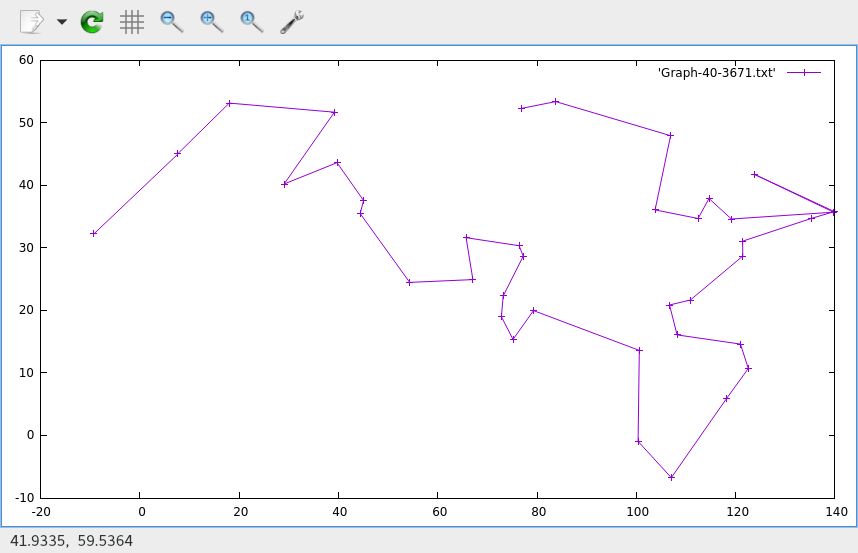
\includegraphics[scale=.60]{Graph40.png}
    \end{figure}\\
    Podemos notar que hay casi ningun cruze en la grafica, lo que quiere decir que esta posiblemente cerca a
    una mejor solucion.\\
    %We can note that one of the most important facts of the representation is that there are practically 0 overlaps of connections. \\
    
    Podemos ver el progreso de la generacion de la solucion en la siguiente grafica:
    %We can also see the progress of the obtaining the optimal solution in the following graph:
    \newpage
    \begin{figure}[h]
        \centering
        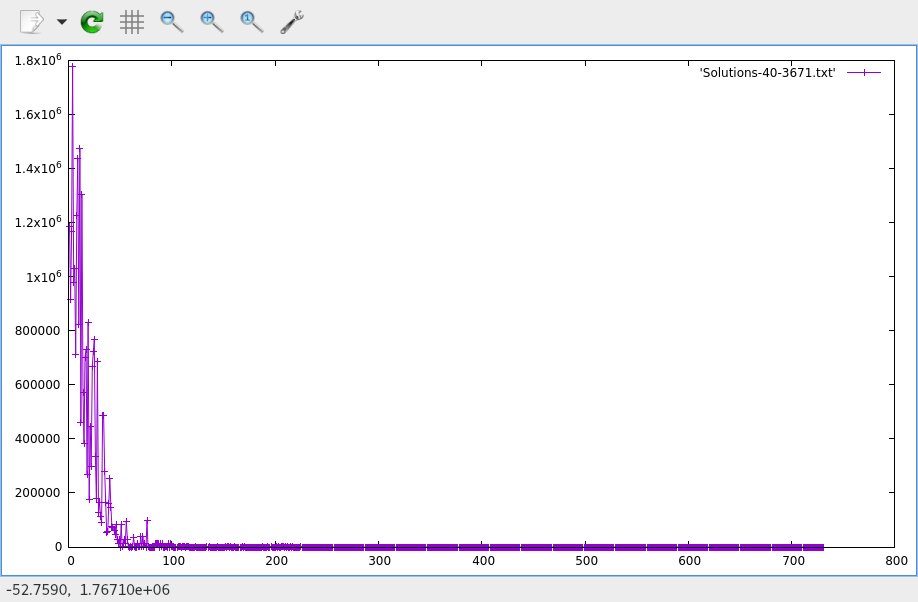
\includegraphics[scale=.35]{Solutions40.png}
    \end{figure}
    Lo que me resalta es que una solucion factible es obtenido relativamente rapido pero la mejora se puede
    ver que es muy poco despues. Para gastar menos tiempo el epsilon que determina cuando termina o 
    el enfiramiento podrian ser ajustado para gastar menos tiempo.\\
    %What stands out is how quickly a possible solution was obtained.After roughly 400 solutions the
    %improvement slowly petered out. To waste less time the epsilon that governed how large the starting
    %temperature would be could probably be lowered. \\
    
    La siguiente grafica solo guarda los minimos globales, pero podemos ver que el numero de mejoras son muy
    pocas en total.
    %The following graph only tracks the global minimum. We can see a similar issue with the temperature in this one. 
    \begin{figure}[h]
        \centering
        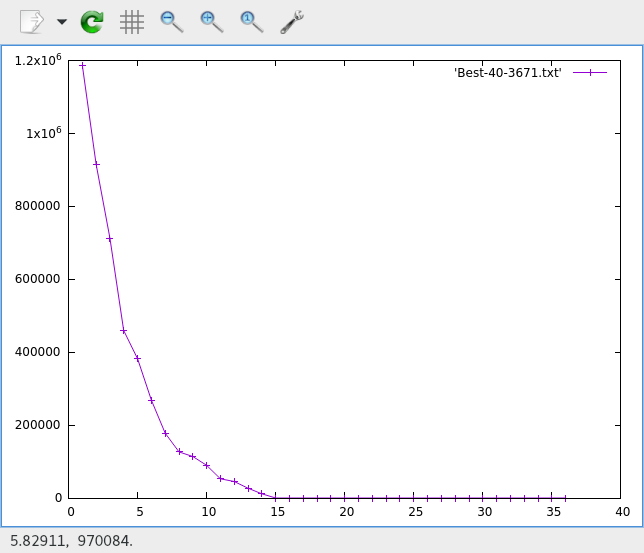
\includegraphics[scale=.42]{Best40.png}
    \end{figure}
    
    Los 5 mejores soluciones de la instancia de 150 de 50 semillas son los siguientes:
    %The best 5 paths for 150 instances from the first 50 seeds are the following:
        \begin{center}
        \begin{tabular}{ |c | c |} 
             \hline
             Semilla & Funcion de Costo \\
             \hline
             10 & 0.22563770969196262 \\ 
             14 & 0.2271077841637491 \\ 
             46 & 0.22743108693616382\\ 
             9 & 0.0.229985277375067\\ 
             12 & 0.2308175880901926\\  
             \hline
        \end{tabular}
    \end{center}
    El mejor semilla resulta en el siguiente camino:
    %With the best Seed resulting in the following solution:
    \begin{center}
    183,340,1038,339,502,12,828,151,822,166,655,819,1073,169,326,328,495,167,494,1037,330,666,818,658,74,1001,
    980,297,336,840,511,662,837,979,493,509,329,839,829,661,657,663,2,172,182,673,496,173,19,667,184,490,344,
    654,665,653,823,7,816,678,187,14,181,982,345,332,26,185,991,27,353,990,981,165,499,984,8,331,995,492,25,501,
    164,504,985,500,825,343,510,660,20,334,999,349,491,347,817,23,988,978,5,1004,676,163,656,832,505,168,9,815,
    508,986,1,507,820,22,351,3,333,4,176,352,668,6,174,489,75,483,652,1075,821,512,179,671,16,520,675,186,826,
    11,1003,674,871,670,350,327,444,17,346,171
    \end{center}
    Que resulta en la siguiente grafica:
    %Which results in the following graph:
    \begin{figure}[h]
        \centering
        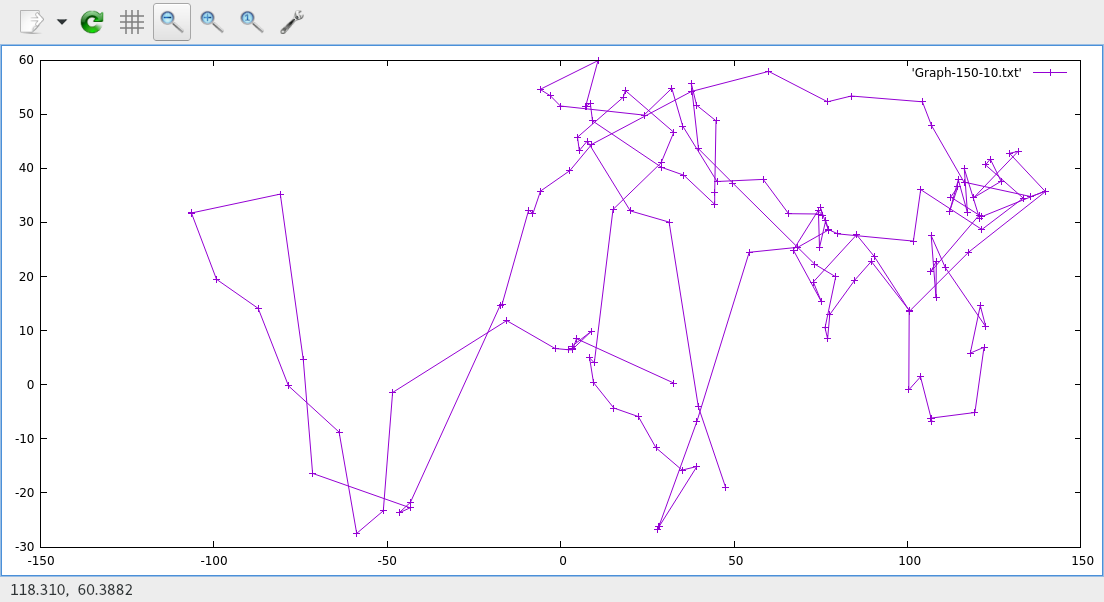
\includegraphics[width=\textwidth,height=\textheight,keepaspectratio]{Graph150.png}
    \end{figure} \\
    Lo que resulta como obvio es que hay demasiados curzes y interseciiones. Lo que creo es que necesita
    mas tiempo para una solucion optima para ser encontrado. Pero no en la temperatura si no en los lotes, ya
    que en las siguientes graficas podemos notar un comportamiento similar a la instancia de 40. Como
    L solo revisa un numero bajo de posible vecinos, incrementar el numero de vecinos revisados podria mejorar
    la calidad de cada lote.\\
    %What can obviously be seen is that there are too many crosses and intersections. The most likely culprit
    %being that more time was needed for an optimal solution to be found. As mentioned previously, L or the 
    %number of better solutions checked in each lot, was set relatively low due to how long it normally took.
    %We can see a similar trend to the instance of 40 cities in the following graphs.\\
    \begin{figure}[H]
        \centering
        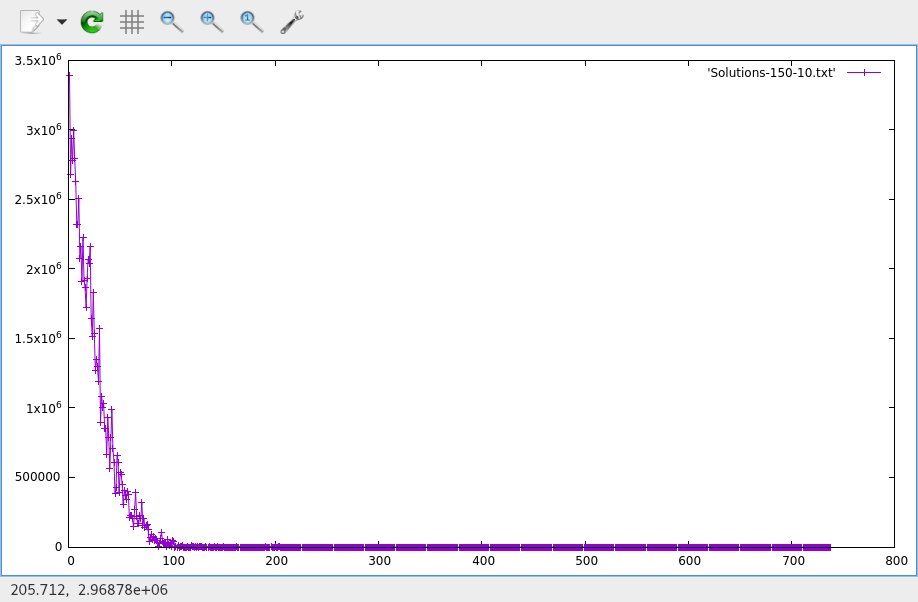
\includegraphics[width=\textwidth,height=\textheight,keepaspectratio]{Solutions150.png}
        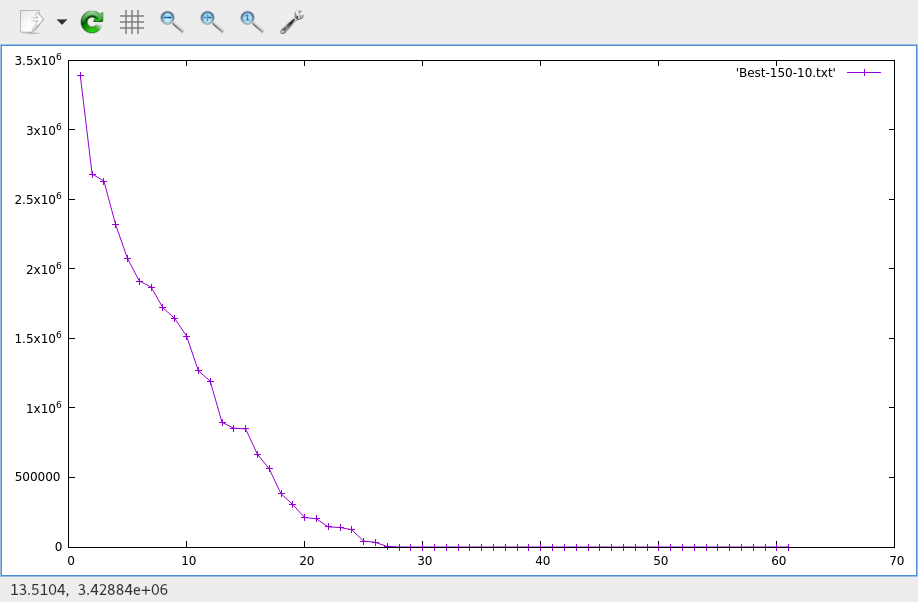
\includegraphics[width=\textwidth,height=\textheight,keepaspectratio]{Best150.png}
    \end{figure}\\
    
    Mejorar la programa se podria ver en ajustar que la temperatura termina mas rapido y que el numero de lotes
    se incrementa. Si se resolve el tiempo de generar una nueva solucion, incrementar L no deberia afectar
    el tiempo de ejecuccion tanto. Como esta el programa, mas grande que esta la instancia pero va a funcionar.
    %To better program I assume increasing the amount that the temperature is cooled one each iteration to
    %save time, as well as increasing L so that each lot is more valuable would make the program better. Fixing
    %the problem with creating a new solution would also allow for more solutions to be tested.
    %%%%%%%%%%%%%%%%%%%%%%%%%%%%%%%%%%%%%%%%%%%%%%%%%%%%%%%%%%%%%%%%%%%%%%%%%%%%%%%%%%%%%%%%%%%%%%%%%%%%%%%%%%
    \section{Bibliography}
    % Bibliografía (TSP, SA/TA, tecnologías usadas) % 
    https://www.quantamagazine.org/computer-scientists-break-traveling-salesperson-record-20201008/\\
    https://en.wikipedia.org/wiki/Travelling\_salesman\_problem\\
    https://en.wikipedia.org/wiki/Simulated\_annealing\\
\end{document}